\section{Metodología}\label{sec-Metodología}
La presente investigación adoptó un enfoque mixto para la creación y
evaluación de ítems para ser aplicados en exámenes que evalúan el área
de Lengua Escrita, siguiendo los principios metodológicos establecidos
por autores clásicos en el campo de la educación y evaluación de
aprendizaje, como \textcite{Bloom1956} y \textcite{Messick1989}, y se incorporaron las
perspectivas sobre diseño de ítems educativos \cite{Haladyna2002}.

En este estudio, con el fin de diseñar ítems, se asignó a cuatro
diseñadores humanos y a la versión 4.0 de ChatGPT \cite{OpenAI2023} el
desarrollo de ítems para evaluar competencias en el área de Lengua
Escrita, siguiendo las teorías de evaluación educativa propuestas por
\textcite{Popham1990}. Se empleó la metodología de triangulación de datos
\cite{Denzin1978} para enriquecer la calidad y confiabilidad de los ítems
mediante la combinación de múltiples perspectivas y fuentes. Cada
diseñador humano fue responsable de la creación de 14 ítems, y ChatGPT
generó 28 ítems, totalizando 84 ítems en el área de Lengua Escrita. La
\Cref{fig01} ilustra este proceso metodológico.


\begin{figure}[htpb]
\centering
\begin{minipage}{\textwidth}
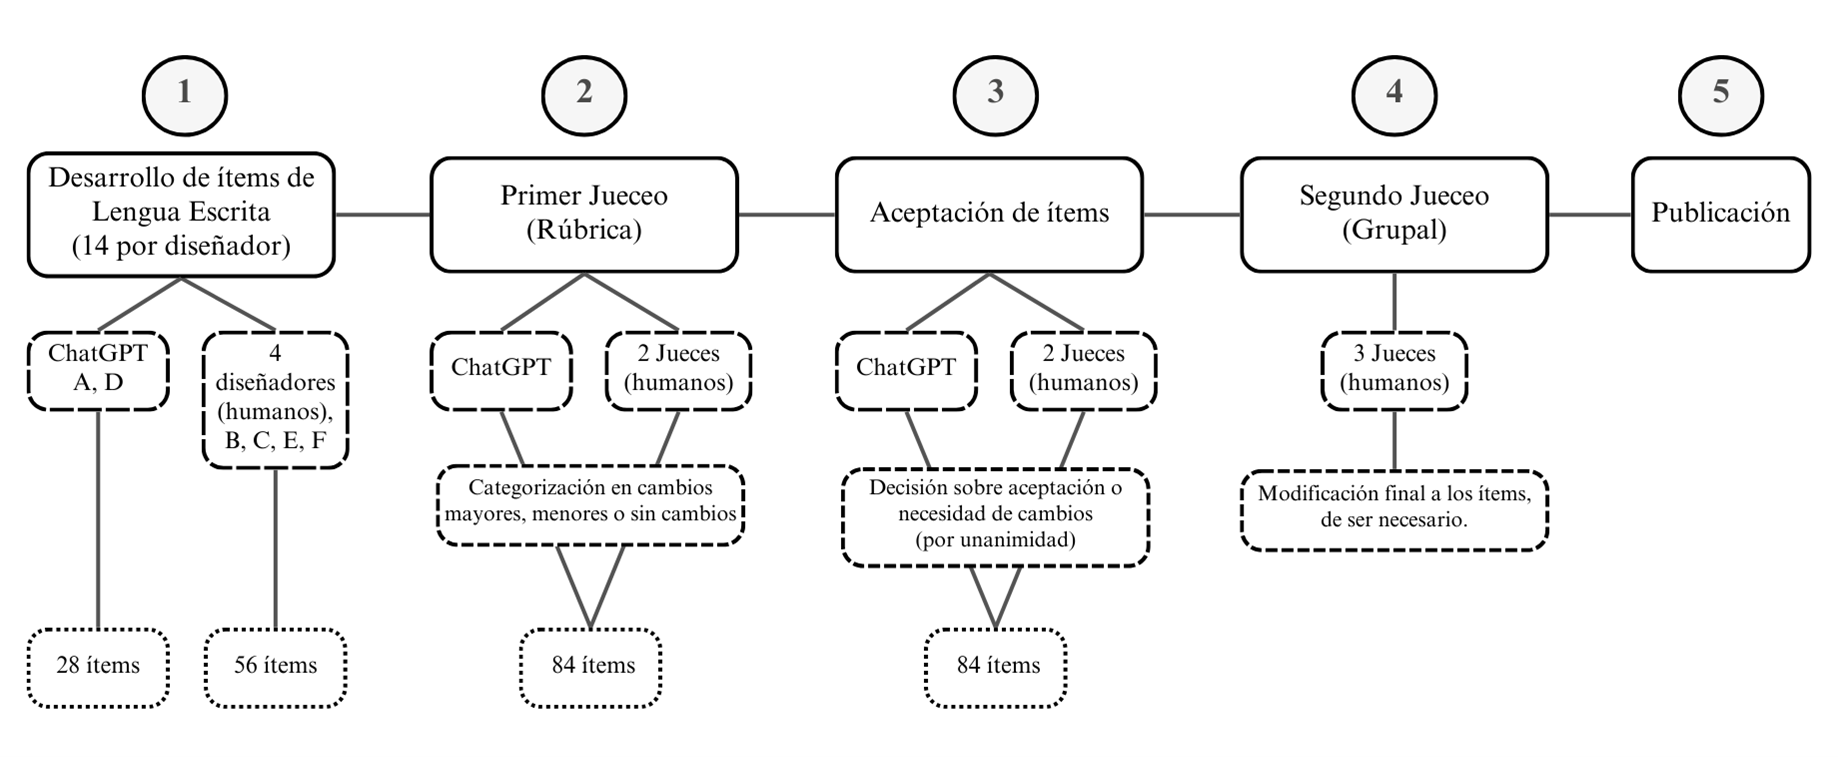
\includegraphics[width=\textwidth]{image1.png}
\caption{Proceso de evaluación y revisión de los ítems.}
\label{fig01}
\source{Elaboración propia.}
\end{minipage}
\end{figure}

Para el desarrollo de ítems se hizo uso de la IAGen ChatGPT
(\url{chat.openai.com}) en su versión de pago nombrada 4.0. Se abrieron
conversaciones por cada ítem creado, ya que todavía no estaba disponible
la posibilidad de crear un GPT con los criterios específicos para la
elaboración de ítems. En este sentido, cada ítem fue solicitado con las
características del manual de Lengua Escrita, comenzando por el uso de
la Taxonomía de \textcite{Anderson2001} para el nivel de demanda
cognitiva según la tabla de especificaciones. En cada prompt creado se
especificó:

\begin{enumerate}
	\def\labelenumi{\arabic{enumi}.}
	\item
	Identificación del contenido a evaluar
	\item
	Descripción del contenido a evaluar:
	
	\begin{enumerate}
		\def\labelenumii{\alph{enumii}.}
		\item
		Interpretación
		\item
		Ejemplos
		\item
		Delimitación del contenido
		\item
		Conocimientos y habilidades previas
		\item
		Actividades cognoscitivas
	\end{enumerate}
	\item
	Plantilla del ítem:
	
	\begin{enumerate}
		\def\labelenumii{\alph{enumii}.}
		\item
		Estructura base del ítem
		\item
		Características del texto
		\item
		Estructura y descripción de respuesta correcta y distractores.
	\end{enumerate}
	\item
	Peculiaridades de la plantilla:
	
	\begin{enumerate}
		\def\labelenumii{\alph{enumii}.}
		\item
		Base del ítem
		\item
		Vocabulario empleado
		\item
		Edición
		\item
		Peculiaridades de los distractores
	\end{enumerate}
	\item
	Bibliografía consultada y a consultar
\end{enumerate}

Por otro lado, la evaluación de los ítems fue realizada por dos jueces
humanos y por ChatGPT, siguiendo el modelo de evaluación de contenido
descrito por \textcite{Haladyna2004} y \textcite{Lynn1986}. Los jueces evaluaron cada
ítem en términos de necesidad de cambios, calidad de distractores y
aceptabilidad general del ítem. Ante esto, es importante resaltar que el
método utilizado para la evaluación de los ítems fue a doble ciego; a
ChatGPT tampoco se le indicó si quien elaboró el ítem era un ser humano
o una IAGen. Este proceso de evaluación se alinea con las
recomendaciones de \textcite{Nitko2011} sobre la importancia de una
revisión integral en la construcción de ítems de evaluación.

Los jueces evaluaron los ítems con una rúbrica (véase \Cref{tab-01}), por lo
que en esta etapa no interactuaron entre sí. Al final debían señalar si
el ítem debiese ser aceptado, aceptado con modificaciones o, bien,
podían descartarlo. Asimismo, a ChatGPT se le solicitó evaluar cada uno
de los ítems con la rúbrica disponible; es importante destacar que era
necesario tener una conversación diferente por cada ítem evaluado,
puesto que su capacidad de recordar la rúbrica era corta; es posible que
en la actualidad haya mejorado, por lo que se tiene que seguir probando
esta herramienta.



\begin{table}[!htpb]
\centering
\small
\caption{Dimensiones de la rúbrica.}
\label{tab-01}
\begin{tabular}{ll}
\toprule
Dimensiones & Elementos Clave \\
\midrule
\multirow{2}{*}{Claridad y Pertinencia del Contenido} & - Información necesaria y clara \\
    & - Tema comprensible para el público objetivo \\
\multirow{2}{*}{Neutralidad y Accesibilidad} & - Libre de sesgos\\
	& - Inclusión de imágenes/gráficas claras \\
\multirow{2}{*}{Concisión y Formato} & - Longitud adecuada del texto\\
		& - Cumplimiento de las especificaciones de formato \\
\multirow{2}{*}{Alineación Curricular} & - Congruencia con especificaciones\\
	& - Adecuación al nivel cognitivo y al público objetivo \\
\multirow{2}{*}{Claridad Disciplinar y Enfoque} & - Brevedad y claridad situacional\\
	& - Presentación directa y positiva \\
\multirow{3}{*}{Redacción y Ortografía} & - Claridad en la redacción\\
	& - Uso de vocabulario y ortografía adecuados\\
	& - Ausencia de sesgos y temas delicados \\
\multirow{3}{*}{Estructura de Respuestas} & - Uniformidad y plausibilidad de las opciones\\
	& - Ausencia de pistas indebidas\\
	& - Consistencia gramatical \\
Formato y Presentación & - Uso correcto de elementos de formato \\
\bottomrule
\end{tabular}
\source{Elaboración propia.}
\end{table}

Los resultados de las evaluaciones reflejaron una gama de decisiones,
desde la aceptación de ítems sin cambios hasta la sugerencia de
modificaciones en menor o mayor grado; o bien, el rechazo del ítem.
Estas decisiones se basaron en criterios establecidos por expertos en
evaluación educativa, como la relevancia, claridad y justicia de los
ítems \cite{Downing2003}.

Además, algunos ítems fueron seleccionados para un segundo jueceo
grupal, reflejando la metodología de revisión colaborativa sugerida por
\textcite{Stiggins2001}, lo cual permite una evaluación más profunda y detallada
en casos donde los ítems presentan desafíos particulares o requieren
ajustes más significativos. En este segundo jueceo se volvió a hacer uso
de la rúbrica, pero escuchando las observaciones de los participantes,
además se añadió a un tercer juez para tener una mejor variedad y
perspectiva sobre el jueceo.

Una vez finalizado este segundo jueceo en versión grupal, se procedió al
proceso de publicación de los ítems en su versión impresa para su
aplicación en el mes de noviembre del año 2023, como parte del proceso
de selección de ingreso a la universidad. En esta aplicación se contó
con la participación de 2,263 sustentantes, siendo 50.06~\% mujeres y
49.93~\% hombres. Los resultados de aplicación del modelo Rasch, el cual
es idóneo para medir actitudes, habilidades o personalidad
\cite{Tristan1998}, se presentan en el \Cref{appdx1}, donde todos los ítems
resultaron con índices favorables conforme a los principios de la Teoría
de Respuesta al Ítem (TRI).

Por otro lado, para el análisis del comportamiento de los jueces se
realizaron los siguientes pasos:

\begin{enumerate}[label=\Alph*)]
\item Para observar las diferencias entre el jueceo a ítems diseñados por humanos y ChatGPT
\begin{enumerate}[label=\arabic*.]
\item Preparación de datos, de forma categórica.
\item Prueba Chi-cuadrado en SPSS, siguiendo las recomendaciones de \cite{Field2013}.
\item Preparación de datos, de forma numérica para proceder a un ANOVA o
bien la prueba de Kruskal-Wallis \cite{Field2013,Howell2012}.
\item Prueba de normalidad en SPSS; el resultado fue no normal, por lo que
se procedió a la prueba de Kruskal-Wallis con las variables: Creadores
(Humano, ChatGPT), Juez A, Juez B, ChatGPT; además se aplicó la prueba
U de Mann-Whitney (Field, 2013) realizando la prueba por cada una de
las variables para revisar si había alguna variación. Todos ellos con
el \emph{software} SPSS.
\item Análisis de resultados con estadísticos básicos comparativos.
\end{enumerate}

\item Para observar la concordancia entre jueces
\begin{enumerate}[label=\arabic*.]
\item Prueba de Kappa de Cohen \cite{McHugh2012}, entre jueces: A y B, A y
ChatGPT, B y ChatGPT, a través del \emph{software} SPSS.
\item Prueba alfa de Krippendorff \cite{Hayes2007}: A, B y ChatGPT, a través del software R (Versión 2023.12.0+369), con	paquetería tidyverse e IRR.
\item Análisis de resultados con estadísticos básicos comparativos.
\end{enumerate}

\end{enumerate}
